
\documentclass{article}

\title{A New Pseudo-Solution of Hydrogen}
\author{Brent Baccala}

\usepackage{amsmath}
\usepackage{amsfonts}

\usepackage{xcolor}
\usepackage{comment}
\usepackage{graphicx}

\usepackage[hidelinks]{hyperref}

\usepackage{tabularx}

\usepackage{longtable}

% For drawing ansatz diagrams

\usepackage{tikz}
\usetikzlibrary{calc}
\usetikzlibrary{positioning}
\usetikzlibrary{fit}
\usetikzlibrary{backgrounds}

\def\coeff{\framebox(10,10){}}
\newcommand{\tikzmark}[1]{\tikz[overlay,remember picture] \node (#1) {};}
\def\R32003{$F_{32003}$}

\begin{document}
\parindent 0pt

\maketitle

\begin{abstract}
The author has developed a novel technique, based on differential algebra,
for finding exact solutions of partial
differential equations.  As an illustration of the method,
I derive a previously unknown exact solution to the simplest time-independent Schr\"odinger equation for hydrogen.
The solution is $J_0(2\sqrt{x+r})$ where $J_0$ is the Bessel function $J_0$, and
the result can be easily verified using Mathematica (p. 18).
\end{abstract}

\parskip 12pt

\subsection*{Introduction}

An January 2023, I discovered a previously unknown solution to the simplest Schrödinger equation for the hydrogen atom.

It turns out that this wavefunction:

\begin{equation}
\Psi = J_0(2\sqrt{x+r})
\end{equation}

where $J_0$ is the ordinary Bessel function $J_0$, solves the Schrödinger equation for hydrogen:

\begin{equation}
-\frac{1}{2}\nabla^2 \Psi - \frac{1}{r}\Psi = E \Psi
\end{equation}

with E=0.

It does not, however, satisfy the global integrability condition required for it to be a valid wavefunction:

\begin{equation}
\int|\Psi|^2 < \infty
\end{equation}

Therefore, it is only a pseudo-solution, since it satisfies the differential equation but is not a valid wavefunction.

A ``proof by Mathematica'' is on page \pageref{verification}.

What I find surprising about the result is that it solves one of the best known equations in mathematical physics, yet has apparently remained undiscovered for over a hundred years!


\subsection*{Schr\"odinger's Equation for Hydrogen}

\begin{comment}
A short list of methods to find exact solutions to PDEs:

\begin{itemize}
\item separation of variables
\item method of characteristics
\item transform methods (Fourier transform on space variables)
\item symmetry methods
\item calculus of variations
\item Evans: Laplace's eq is invariant under rotations, so look for functions of r; this is a variant of sep of var
\item Evans: Poisson's eq: Green's function is constructed from radially symmetric solution to Laplace's eq
\item Evans: Poisson's eq: calculus of variations; show that solution minimizes a functional
\item Evans: heat eq: uses several scaling symmetries to justify solution form depending on a single expression
\item Evans: Duhamel's principle: separate out one variable (t) that appears like $u_t - Lu = f$ (L has no time deriv);
      form the ``retarded solution'' that represents the effect of an infinitesimal $f$, then integrate over time
\item Evans: heat eq: scaling symmetry $\rightarrow$ fundamental sol $\rightarrow$ convolution to handle arbitrary initial condition
      $\rightarrow$ Duhamel's principle to handle the inhomogenous component
\end{itemize}
\end{comment}

\begin{comment}
A short list of methods to find exact solutions to PDEs includes separation of variables,
the method of characteristics, transform methods (including Fourier transforms),
symmetry methods, Green's functions, Duhamel's principle, and the calculus of variations.
The author has developed another exact solution technique based on differential algebra
and has used it to find a new solution to one of the most well-studied equations
in mathematical physics, the Schr\"odinger equation for hydrogen.
\end{comment}

The Schr\"odinger equation is the quantum mechanical analog of Newton's second law.
Both Newton's equation and Schr\"odinger's equation
describe the time evolution of a system
of particles interacting under the influence of forces.
Newton's classical second law $F=ma$
describes the time evolution of the position and velocity of each particle.
Schr\"odinger's quantum mechanical formulation $H\Psi=i\frac{\delta}{\delta t} \Psi$
describes the time evolution
of the wavefunction $\Psi$, which is a complex-valued function of particle positions
that encodes a probability density function for
the particle positions as $|\Psi|^2$ and a probability density function
for the particle momenta as its Fourier transform $|\hat{\Psi}|^2$.

There is no one Schr\"odinger equation any more than there is one $F=ma$.
Each physical system under consideration gives rise to a different collection
of particles and interacting forces, and a different Hamiltonian operator $H$.
Indeed, even the approximations we
make strongly determine the form of the equation for a given system.

The Hamiltonian operator $H$, so named because of its connection to Hamiltonian
mechanics, is most typically given in the form $H=T-V$, where $T$ is the
sum of the kinetic energy of all particles and $V$ is the potential energy
of the system, due to its forces.

\begin{equation*}
H=T-V
\end{equation*}

One of the simplest Schr\"odinger equations is for the hydrogen atom,
considering the electric force attraction between the nucleus and
the electron, and ignoring all other effects.  It has the following form:

\begin{equation*}
%\label{schrodinger}
-\frac{1}{2}\nabla^2 \Psi - \frac{1}{r}\Psi = i \frac{\delta}{\delta t} \Psi
\end{equation*}

where $\Psi$ is the wavefunction, $\nabla^2$ is the Laplacian,
and $r$ is the distance between the two particles.  We use Hartree atomic units,
a system of units in which four fundamental physical constants\footnote{the reduced Planck
constant, the elementary charge, the electron mass, and the Coulumb constant} are
assigned the value of 1, in order to eliminate the need for any
physical constants in the equation.  The unit of distance, in particular,
is {\it Bohr radii}, approximately half an angstrom (\AA = $10^{-10}$ m).
The first term, $-\frac{1}{2}\nabla^2 \Psi$,
is the kinetic energy operator, and the second term, $-\frac{1}{r}\Psi$, is
the potential energy term.

We can further simplify the general, time-dependent Schr\"odinger equation
by requiring that the position and momentum probability density functions
each be time-independent.  This restricts the solution to stable states
of the hydrogen atom, settles the wavefunction up to a multiple of $e^{itE}$,
where $E$ is the state's energy in Hartrees (approximately 27 eV),
and leads to the time-independent Schr\"odinger equation for hydrogen:

\begin{equation}
\label{schrodinger hydrogen}
-\frac{1}{2}\nabla^2 \Psi - \frac{1}{r}\Psi = E \Psi
\end{equation}

This equation is amenable to seperation of variables.
Using spherical coordinates and writing $\Psi$ as $\Psi=R(r)Y(\theta, \psi) = R(r)P(\theta)F(\psi)$,
substituting into \eqref{schrodinger hydrogen}, we obtain the following expansion\footnote{hyperphysics}:

\begin{equation*}
\frac{1}{R} \frac{d}{dr}\left[ r^2 \frac{dR}{dr}\right] + 2(Er^2 + r)
+ \left[\frac{1}{P\sin\theta} \frac{d}{d\theta}\left[\sin\theta\frac{dP}{d\theta}\right]+\frac{1}{F\sin^2\theta}\frac{d^2 F}{d\psi^2}\right] = 0
\end{equation*}

The first part, dependant on $r$, is the {\it radical equation}, whose solutions are, in general.
hypergeometric functions, but which, in the case of specific energy values,
simplify to polynomials in $r$
times an exponential of $r$.  It is these solutions, combined with the solution
of the second part of the equation (the colatitude equation, solved by the associated Laguerre polynomials,
and the azimuthal equation), which have been known for a hundred years, and are
hence referred to as the {\it classical solutions} to hydrogen.

\begin{figure}
\begin{center}
\begin{tabular}{ccc}
{\bf Energy}		& {\bf Wavefunction}		& {\bf Shell} \\
{\bf (Hartrees)}	& & \\
\\
$-\frac{1}{2}$		& $e^{-r}$			& 1s \\
$-\frac{1}{8}$		& $(2-r)e^{-r/2}$		& 2s \\
			& $xe^{-r/2}$			& 2p \\
			& $ye^{-r/2}$			\\
			& $ze^{-r/2}$			\\
$-\frac{1}{18}$		& $(27-18r+2r^2)e^{-r/3}$	& 3s \\
			& $(6-r)xe^{-r/3}$		& 3p \\
			& $(6-r)ye^{-r/3}$		\\
			& $(6-r)ze^{-r/3}$		\\
%%			& $(xy)e^{-r/3}$		& 3d \\
\end{tabular}
\end{center}
\end{figure}

The associated energy levels are negative because these are bound states.  Zero energy
would correspond to an electron and a proton at rest an (infinitely) large distance apart.

The classical solutions are separable and square integrable
and are each paired with a negative energy value, of which $-\frac{1}{2}$ is the lowest,
and corresponds to the 1s or ground state.

Yet the existance of separable solutions leaves open the existance of non-separable solutions.

It is perhaps surprising that such a well-studied equation would have fairly simple, previously
undiscovered, non-separable solutions.

\subsection*{Differential Reduction Step}

I attempted to use the Rosenfeld-Gr\"obner algorithm to reduce equation \eqref{schrodinger hydrogen}
modulo \eqref{ansatz 5}, but it ultimately ran out of memory on a 96 GB computer after
30 hours.  Instead, I used Sage to construct a polynomial ring modulo the ideal
$r^2-x^2-y^2-z^2$ to handle the algebraic extension (present not in the ansatz proper,
but in the original ring used to construct the PDE).  Next I directed the software
to expand the derivatives in \eqref{schrodinger hydrogen} and substitute for $\Psi''$ and $v$
according to the ansatz \eqref{ansatz 5}.  The result is
a rational function
with a 228 term numerator and an 18 term denominator.  We ignore the denominator.  The numerator begins:

% I used a Sage-based computer program with the following ansatz.
\begin{comment}
I found this solution roughly as follows.\footnote{
I discovered an alternate form of this solution using a somewhat more complex ansatz
on January 24, 2023.  By January 26, I had established the solution in its current form.
The original ansatz produced a rational function with
a 1254 term numerator and a 36 term denominator, that gave rise to a system of 224 equations,
and was first solved using numerical approximation (scipy.optimize.root).
}

Use Cartesian coordinates.  Let $v$ be a linear polynomial in the coordinates and the root $r=\sqrt{x^2+y^2+z^2}$,
Reduce the input PDE \eqref{schrodinger} modulo differential ideal \eqref{ansatz 5}, obtaining
\end{comment}

\begin{equation}
\label{schrodinger modulo ansatz 5}
%% -8r\Psi x^5 b_1 b_2^2 n_1 - r\Psi x^5 b_1 b_4^2 n_1 - r \Psi x^5 b_1 b_6^2 n_1 - 2r\Psi x^5 b_2 b_3 b_4 n_1 - \cdots
-2r\Psi x^3 E d_1 v_1 - 3r\Psi x^3 n_1 v_0^2 v_1 - r\Psi x^3 n_1 v_1^3 - r\Psi x^3 n_1 v_1 v_2^2 - r\Psi x^3 n_1 v_1 v_3^2 - \cdots
\end{equation}

In this run of the program, I was using different names for the constants than
I use in the paper.  $d_i$, $m_i$, $n_i$ instead of $a_i$, $b_i$, $c_i$.

\subsection*{Projection Step}

Having reduced our PDE \eqref{schrodinger hydrogen} by the differential ideal defined by \eqref{ansatz 5},
we now wish to project our solution onto the subspace of the constants.  We're looking for
constants that will solve equation \eqref{schrodinger modulo ansatz 5} for all values of $x$, $y$, $z$, $r$,
$\Psi$, and $\Psi'$, so
we collect like terms in $x$, $y$, $z$, $r$, $\Psi$, and $\Psi'$, organizing the numerator like this:

\begin{equation}
%%\left(-8 b_1 b_2^2 n_1 - b_1 b_4^2 n_1 - b_1 b_6^2 n_1 - 2 b_2 b_3 b_4 n_1 - 2b_2 b_5 b_6 n_1 \right) r\Psi x^5 - \cdots
r\Psi x^3 \left(-2 E d_1 v_1 - 3 n_1 v_0^2 v_1 - n_1 v_1^3 - n_1 v_1 v_2^2 - n_1 v_1 v_3^2\right) - \cdots
\end{equation}

The expressions in parenthesis gives us a system of equations (only one is shown)
involving the $v_i$, $d_i$, $m_i$ and $n_i$ variables that, if satisfied,
will yield a solution to \eqref{schrodinger hydrogen} in the form \eqref{ansatz 5}.  Once
duplicate equations are dropped, the system has 34 equations.


%%sage: latex(matrix(eqns()).transpose())
\begin{equation}
\label{polynomial system}
\begin{array}{r}
-2 \, n_{1} v_{0}^{3} - 4 \, n_{1} v_{0} v_{1}^{2} - 4 \, n_{1} v_{0} v_{2}^{2} - 2 \, n_{1} v_{0} v_{3}^{2} - 4 \, E d_{1} v_{0} \\
-2 \, n_{1} v_{0}^{3} - 4 \, n_{1} v_{0} v_{1}^{2} - 2 \, n_{1} v_{0} v_{2}^{2} - 4 \, n_{1} v_{0} v_{3}^{2} - 4 \, E d_{1} v_{0} \\
-2 \, n_{1} v_{0}^{3} - 2 \, n_{1} v_{0} v_{1}^{2} - 4 \, n_{1} v_{0} v_{2}^{2} - 4 \, n_{1} v_{0} v_{3}^{2} - 4 \, E d_{1} v_{0} \\
-4 \, m_{1} v_{0} v_{1} v_{2} \\
-4 \, m_{1} v_{0} v_{1} v_{3} \\
-4 \, m_{1} v_{0} v_{2} v_{3} \\
-4 \, n_{1} v_{0} v_{1} v_{2} \\
-4 \, n_{1} v_{0} v_{1} v_{3} \\
-4 \, n_{1} v_{0} v_{2} v_{3} \\
-3 \, m_{1} v_{0}^{2} v_{1} -  \, m_{1} v_{1}^{3} -  \, m_{1} v_{1} v_{2}^{2} -  \, m_{1} v_{1} v_{3}^{2} \\
-3 \, m_{1} v_{0}^{2} v_{2} -  \, m_{1} v_{1}^{2} v_{2} -  \, m_{1} v_{2}^{3} -  \, m_{1} v_{2} v_{3}^{2} \\
-3 \, m_{1} v_{0}^{2} v_{3} -  \, m_{1} v_{1}^{2} v_{3} -  \, m_{1} v_{2}^{2} v_{3} -  \, m_{1} v_{3}^{3} \\
-2 \, m_{1} v_{0}^{3} - 4 \, m_{1} v_{0} v_{1}^{2} - 4 \, m_{1} v_{0} v_{2}^{2} - 2 \, m_{1} v_{0} v_{3}^{2} \\
-2 \, m_{1} v_{0}^{3} - 4 \, m_{1} v_{0} v_{1}^{2} - 2 \, m_{1} v_{0} v_{2}^{2} - 4 \, m_{1} v_{0} v_{3}^{2} \\
-3 \, n_{1} v_{0}^{2} v_{1} -  \, n_{1} v_{1}^{3} -  \, n_{1} v_{1} v_{2}^{2} -  \, n_{1} v_{1} v_{3}^{2} - 2 \, E d_{1} v_{1} \\
-3 \, n_{1} v_{0}^{2} v_{2} -  \, n_{1} v_{1}^{2} v_{2} -  \, n_{1} v_{2}^{3} -  \, n_{1} v_{2} v_{3}^{2} - 2 \, E d_{1} v_{2} \\
-3 \, n_{1} v_{0}^{2} v_{3} -  \, n_{1} v_{1}^{2} v_{3} -  \, n_{1} v_{2}^{2} v_{3} -  \, n_{1} v_{3}^{3} - 2 \, E d_{1} v_{3} \\
-2 \, m_{1} v_{0}^{3} - 2 \, m_{1} v_{0} v_{1}^{2} - 4 \, m_{1} v_{0} v_{2}^{2} - 4 \, m_{1} v_{0} v_{3}^{2} \\
- \, n_{0} v_{0}^{2} -  \, n_{0} v_{1}^{2} -  \, n_{0} v_{2}^{2} -  \, n_{0} v_{3}^{2} - 2 \, E d_{0} - 2 \, d_{1} v_{0} \\
-2 \, n_{0} v_{0} v_{1} - 2 \, d_{1} v_{1} \\
-2 \, n_{0} v_{0} v_{2} - 2 \, d_{1} v_{2} \\
-2 \, n_{0} v_{0} v_{3} - 2 \, d_{1} v_{3} \\
-2 \, d_{1} v_{0} v_{1} - 2 \, m_{0} v_{0} v_{1} \\
-2 \, d_{1} v_{0} v_{2} - 2 \, m_{0} v_{0} v_{2} \\
-2 \, d_{1} v_{0} v_{3} - 2 \, m_{0} v_{0} v_{3} \\
- \, n_{1} v_{0}^{3} - 3 \, n_{1} v_{0} v_{1}^{2} -  \, n_{1} v_{0} v_{2}^{2} -  \, n_{1} v_{0} v_{3}^{2} - 2 \, E d_{1} v_{0} \\
- \, n_{1} v_{0}^{3} -  \, n_{1} v_{0} v_{1}^{2} - 3 \, n_{1} v_{0} v_{2}^{2} -  \, n_{1} v_{0} v_{3}^{2} - 2 \, E d_{1} v_{0} \\
- \, n_{1} v_{0}^{3} -  \, n_{1} v_{0} v_{1}^{2} -  \, n_{1} v_{0} v_{2}^{2} - 3 \, n_{1} v_{0} v_{3}^{2} - 2 \, E d_{1} v_{0} \\
-2 \, d_{1} v_{0}^{2} -  \, m_{0} v_{0}^{2} -  \, m_{0} v_{1}^{2} -  \, m_{0} v_{2}^{2} -  \, m_{0} v_{3}^{2} \\
-2 \, d_{0} \\
-2 \, d_{0} v_{0} \\
- \, m_{1} v_{0}^{3} - 3 \, m_{1} v_{0} v_{1}^{2} -  \, m_{1} v_{0} v_{2}^{2} -  \, m_{1} v_{0} v_{3}^{2} \\
- \, m_{1} v_{0}^{3} -  \, m_{1} v_{0} v_{1}^{2} - 3 \, m_{1} v_{0} v_{2}^{2} -  \, m_{1} v_{0} v_{3}^{2} \\
- \, m_{1} v_{0}^{3} -  \, m_{1} v_{0} v_{1}^{2} -  \, m_{1} v_{0} v_{2}^{2} - 3 \, m_{1} v_{0} v_{3}^{2}
\end{array}
\end{equation}

\subsection*{Prime Decomposition}

\begin{comment}
I used a numerical algorithm to solve the system of equations in expectation
of it being faster for larger systems, but the system \eqref{polynomial system}
is small enough that exact methods are usable.
\end{comment}
\eqref{polynomial system} is simple enough that we can form
an ideal $I$ in $\mathbf{Q}[v_0,...,m_1,E]$ from \eqref{polynomial system}, and
Sage can calculate a Gr\"obner basis for the radical $I$ in less than a second.
While we could work with the Gr\"obner basis directly\footnote{A Gr\"obner basis
of the solution ideal in lexicographic order $E>d_i>m_i>n_i>v_i$ contains 65 polynomials.}
, I find it more
useful to study the primary decomposition, which Sage computes using
the Shimoyama-Yokoyama algorithm\footnote{Localization and Primary Decomposition of
Polynomial Ideals, {\it J. Symbolic Computation} (1996) {\bf 22}, 247–277}
as implemented in Singular.  Gr\"obner basis calculations are done
as a subalgorithm of Shimoyama-Yokoyama.

Taking the radical of the ideal simplifies both the theory and the application,
and can be justified because there are no nilpotent elements in our solution
space, which is just 11-dimensional complex space ${\mathbf C}^{11}$.  The
primary decomposition of a radical ideal is also a prime decomposition,
as the distinction between primary and prime ideals is only significant
for non-radical ideals with nilpotent elements.  Sage/Singular computes
the following decomposition into prime ideals:

\begin{verbatim}
sage: I.radical().primary_decomposition()
\end{verbatim}

\begin{subequations}
\label{ideal}
\begin{align}
& \left(n_{1}, n_{0}, m_{1}, m_{0}, d_{1}, d_{0}\right)\label{ideal:5} \\
& \left(v_{3}, v_{2}, v_{1}, v_{0}, d_{0}\right)\label{ideal:4}\\
& \left(v_{1}^{2} + v_{2}^{2} + v_{3}^{2}, v_{0}, d_{1}, d_{0}\right)\label{ideal:3}\\
& \left(v_{3}, v_{2}, v_{1}, m_{1}, m_{0} - n_{0} v_{0}, 2 d_{1} + n_{0} v_{0}, d_{0}, E n_{0} - n_{1} v_{0}\right)\label{ideal:2}\\
& \left(v_{0}^{2} - v_{1}^{2} - v_{2}^{2} - v_{3}^{2}, n_{1}, m_{1}, m_{0} - n_{0} v_{0}, d_{1} + n_{0} v_{0}, d_{0}, E\right)\label{ideal:1}
\end{align}
\end{subequations}

Several of these varieties solve the system of equations, but do not lead to a meaningful solution to the differential equation.
In brief,

\begin{itemize}
\item[\eqref{ideal:5}] sets all coefficients of the ODE to zero, so we discard it,
\item[\eqref{ideal:4}] sets the variable $v$ to zero, so we discard it,
\item[\eqref{ideal:3}] sets the coefficient of
%$\frac{d^2\Psi}{dv^2}$
$D^2\Psi$
in the ODE to zero, resulting in a first-order ODE, so we discard it, too,
\item[\eqref{ideal:2}] corresponds to the classical solutions (see below), and
\item[\eqref{ideal:1}] gives us our new solution (see below).

\end{itemize}

How to understand ideal \eqref{ideal:2}?  $d_0$ is an ideal generator,
so $d_0=0$, and we can always multiply our homogenous differential polynomial by a constant without affecting our result, so we can set $d_1=1$.
Likewise, we can multiply our variable $v$ by a constant and that will only change our coefficients by constants,
and $v_1=v_2=v_3=0$, so we can normalize by setting $v_0=1$.  This simplifies ideal \eqref{ideal:2} to:

\begin{equation}
\left(v_{3}, v_{2}, v_{1}, v_{0} - 1, n_{0} + 2, m_{1}, m_{0} + 2, d_{1} - 1, d_{0}, 2 E + n_{1}\right)
\end{equation}

\begin{equation}
\label{classical eq in ideal}
\begin{gathered}
v=r \\
v \Psi'' + 2 \Psi' + 2(1 + E v) \Psi = 0
\end{gathered}
\end{equation}

This is the classical radial equation obtained by seperation of variables\footnote{See
Pauling and Wilson or
\url{http://hyperphysics.phy-astr.gsu.edu/hbase/quantum/hydrad.html}}.  We use
spherical coordinates, set $\Psi = R(r)P(\theta)F(\psi)$, and obtain the above equation for $R(r)$,
though it is more commonly written in this form:

\begin{equation}
\frac{1}{R} \frac{d}{dr}\left[ r^2 \frac{dR}{dr}\right] + 2(Er^2 + r) = l(l+1)
\end{equation}

where $l$ is the orbital quantum number, which can be zero.  Set $l=0$, $v=r$ and $\Psi=R$ and
expand out the derivative to obtain \eqref{classical eq in ideal}.  Its presence here was
expected and won't be commented on further.

Ideal \eqref{ideal:1} was not expected, and contains our new solution.
$d_0$ is an ideal generator,
so $d_0=0$, and we can set $d_1=1$, by the same logic as above.
Our coordinates are in real space, so our $v_i$ coefficients must be real (why?), so all of their squares must
be positive, and since $v_0^2-v_1^2-v_2^2-v_3^3=0$, $v_0$ must be non-zero.  So we can normalize by setting $v_0=1$.
That simplifies \eqref{ideal:1} to this ideal:

\begin{equation}
\left(v_{1}^{2} + v_{2}^{2} + v_{3}^{2} - 1, v_{0} - 1, n_{1}, n_{0} + 1, m_{1}, m_{0} + 1, d_{1} - 1, d_{0}, E\right)
\end{equation}

This ideal corresponds to the following system of equations:

\begin{equation}
\begin{gathered}
E = 0 \\
d_0 = 0 \qquad
d_1 = 1 \\
m_0 = -1 \qquad
m_1 = 0 \\
n_0 = -1 \qquad
n_1 = 0 \\
v_0 = 1 \qquad
v_1^2 + v_2^2 + v_3^2 = 1
\end{gathered}
\end{equation}

Substituting these values back into our ansatz, we conclude that $\Psi(v)$
is a solution of \eqref{schrodinger} under these conditions:

\begin{equation}
\label{related solution}
\begin{gathered}
v \frac{\delta^2\Psi}{\delta v^2} + \frac{\delta\Psi}{\delta v} + \Psi = 0 \\
v = v_1 x+ v_2 y+ v_3 z+r \\
v_1^2 + v_2^2 + v_3^2 = 1
\end{gathered}
\end{equation}

The expression $v_1 x + v_2 y + v_3 z$ is easily identified as a dot product between
the coordinate $(x,y,z)$ and the unit vector $(v_1, v_2, v_3)$ (remembering
that $v_1^2 + v_2^2 + v_3^2 = 1$).  The direction of this vector is arbitrary,
so we can orient the $x$-axis in this direction and set $(v_1, v_2, v_3) = (1,0,0)$
without loss of generality.

We now have to solve a second order ODE:

\begin{equation}
v \Psi''(v) + \Psi'(v) + \Psi(v) = 0
\end{equation}

Wolfram Mathematica\footnote{I originally used Wolfram Alpha} can now
analyze this equation and determine that it is equivalent
to the Bessel function \eqref{solution}.

\includegraphics[page=1, clip, trim=1in 9in 1in 1in, width=\textwidth]{find Bessel solution.pdf}

leading to...

\vfill\eject

\subsection*{The Main Result}
\parskip 0pt

Consider the following simple Sch\"odinger equation for the hydrogen atom:

\begin{equation}
\label{schrodinger}
-\frac{1}{2}\nabla^2 \Psi - \frac{1}{r}\Psi = E \Psi
\end{equation}

Let $J_0$ be the ordinary Bessel function $J_0$, and set

\begin{equation}
\label{solution}
\Psi = J_0(2\sqrt{x+r})
\end{equation}

where $x,y,z$ are Cartesian coordinates and $r=\sqrt{x^2+y^2+z^2}$.

\vskip 12pt

Then \eqref{solution} is an exact solution to \eqref{schrodinger}, with $E=0$.

\subsection*{Verification}

\label{verification}
The result can be easily verified using Mathematica\footnote{A manual verification is presented in an appendix}, as follows:

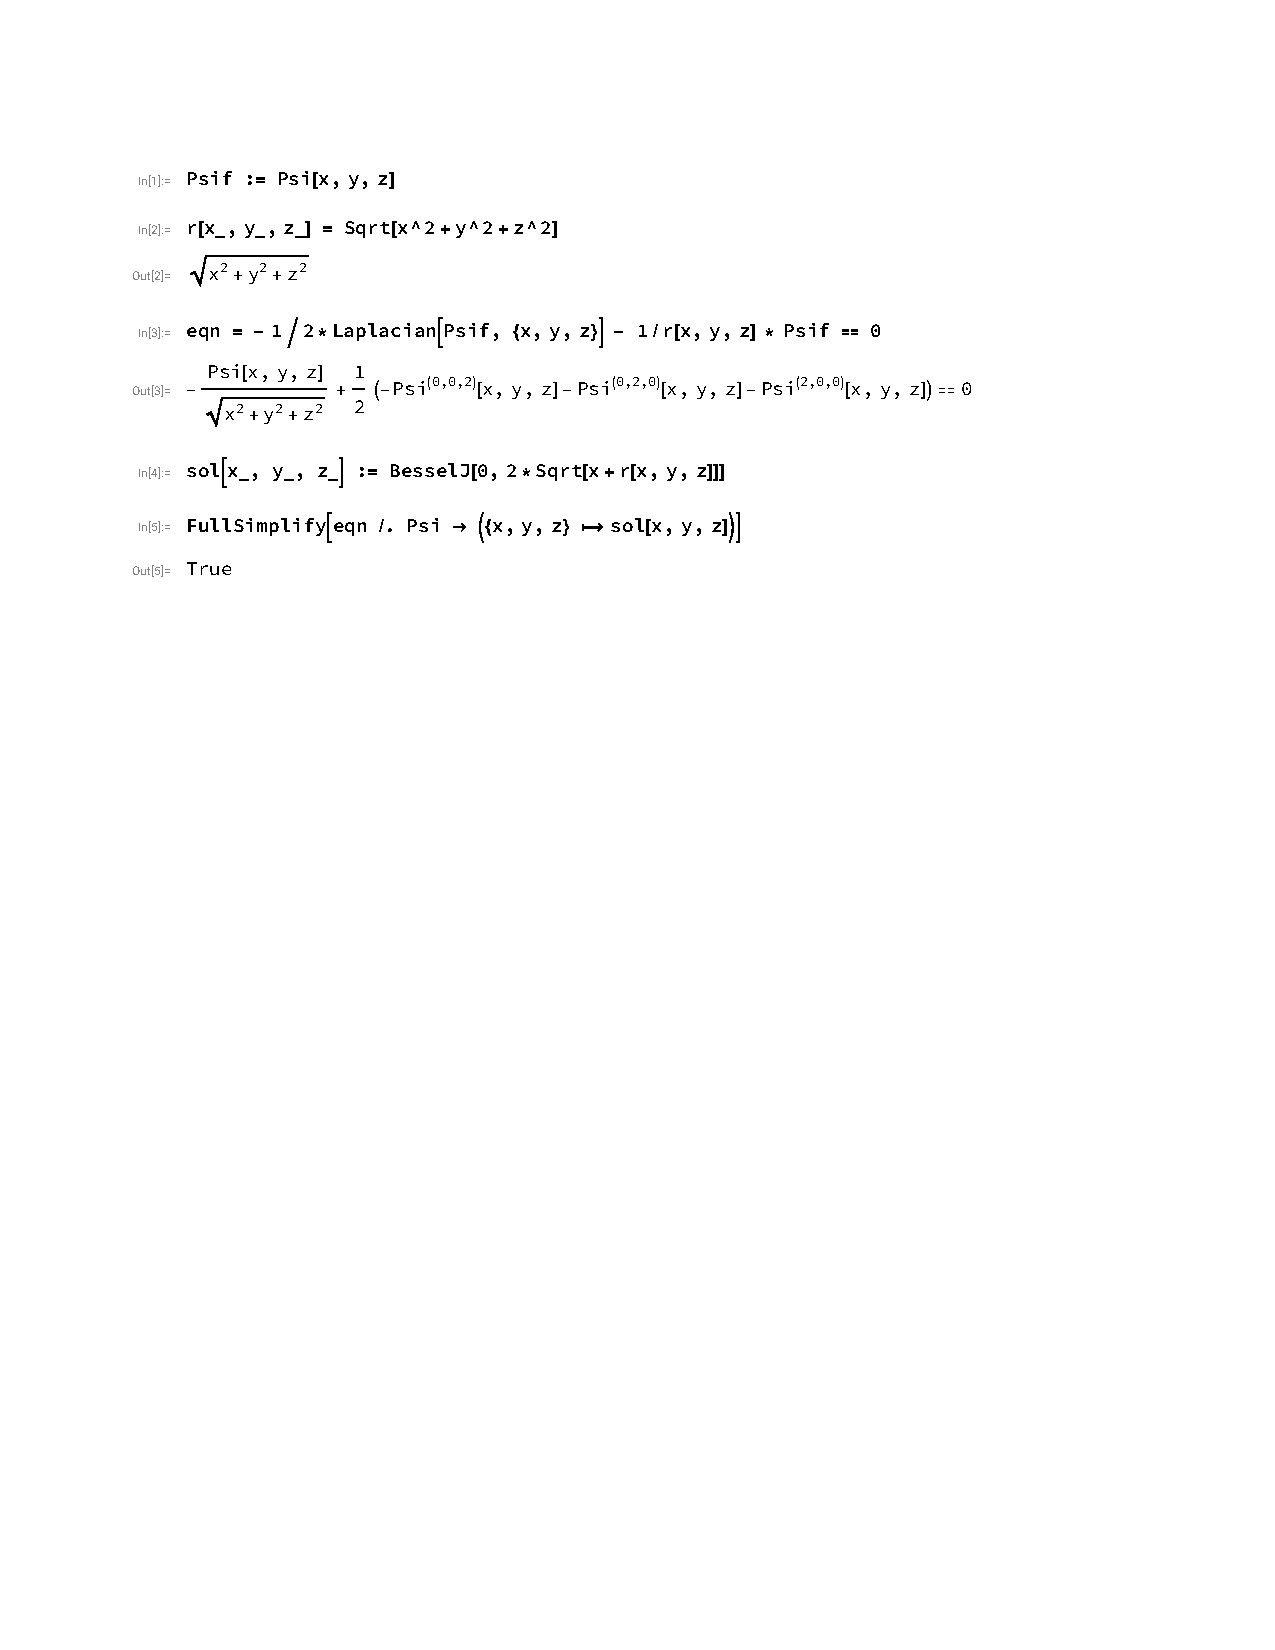
\includegraphics[page=1, clip, trim=1in 7in 1in 1in, width=\textwidth]{improved.pdf}

\subsection*{Generalization}
\parskip 12pt

The choice of $x$ is arbitrary, and any ordinary Bessel function can be used:

\begin{equation}
\label{generalized solution}
\Psi = F(2\sqrt{a_1 x+ a_2 y+ a_3 z+r})
\end{equation}

where

\begin{equation*}
a_1^2+a_2^2+a_3^2=1
\end{equation*}

and $F$ is any linear combination of the Bessel functions $J_0$ and $Y_0$.

\vskip 12pt

Any finite linear combination of functions of the form \eqref{generalized solution} also solves \eqref{schrodinger}.

\subsection*{Software}

The program used to construct the system of equations is available here:

\centerline{\url{https://github.com/BrentBaccala/helium}}

It's a Sage script that works fine with Sage 9.0 on Ubuntu 20.

%Use it to find the witness point \eqref{witness point} by
%running Sage as follows:
Use it to find ideal \eqref{ideal} by
running Sage as follows:

\begin{verbatim}
load('helium.sage')     # loads the script
prep_hydrogen(5)        # select PDE:hydrogen and ansatz:5
init()                  # finish setting everything up
I=ideal(eqns_RQQ)       # constuct ideal from equations
I.radical().primary_decomposition()
\end{verbatim}

Here are some other convenient variables and functions in the script:

\begin{verbatim}
A, B, C, V              # trial forms of various polynomials
eq_a                    # the PDE in its original form
R                       # polynomial ring over integers
F                       # fraction field of R
F_eq_a                  # the PDE modulo the ansatz
F_eq_a_n                # expanded numerator (in R)
F_eq_a_d                # expanded denominator (in R)
eqns_RQQ                # system of equations to solve
\end{verbatim}

%%\section*{Current Implementation Status}
\subsection*{Current Implementation Status}

The algorithm presented above can be used to check any PDE to see if any of its solutions
can be expressed using an ODE structured according to a specific ansatz.  This technique
is complementary to separation of variables, where we check a PDE to see if any of
its solutions can be expressed as a product of factors, each depending on only
a single variable.

As my primary interest lies in quantum mechanics, I have investigated the PDEs
that model hydrogen and helium.

For hydrogen, the PDE is $\nabla^2 \Psi - \frac{1}{r} \Psi = E \Psi$

For helium, the PDE is $\nabla_1^2 \Psi + \nabla_2^2 \Psi - \frac{2}{r_1} - \Psi \frac{2}{r_2} - \Psi \frac{1}{r_{12}} \Psi = E \Psi$,
where $\Psi=\Psi(r_1,r_2,r_{12})$ and $\nabla_i$ is the Laplacian with respect to the $i^{\rm th}$ electron.
$\Psi$ is assumed to have no angular dependence, which has been known since
at least the time of Hylleraas to be a valid assumption for the ground state.

In both cases, I use Hartree atomic units to render the equations dimensionless.

\begin{comment}
Once the PDEs have been reduced modulo the differential ideal corresponding to a selected ansatz,
the resulting system of polynomial equations must be solved.  The major techniques available are:

\begin{enumerate}
\item Exact primary decomposition

This requires the computation of Gr\"obner bases, which often fails due to memory exhaustion
(oom - out of memory) and the limitations of current

\item Numerical approximation (gradient descent / Levenberg-Marquardt)

This requires extraneous ideals/varieties to be removed as they are identified.
I'm currently exploring this approach, as it is the fastest of the three,
using the DHOST algorithm to compute Euclidean Distance polynomials for
identified varieties and use this information to drive the solutions
away from identified varieties in an attempt to find new ones.

Note that this approach, while faster than the others, will never guarantee that all solutions
to the polynomial system have been found.

\item Homotopy continuation

Bertini is a major software program, but Macaulay 2 also supports homotopy continuation.
This technique is slow but, in principle, will identify all irreducible varieties.
In practice, Bertini did not identify all five irreducible varieties for hydrogen Ansatz 5.
\end{enumerate}

\end{comment}

\subsection*{Conclusion}

As we've seen, using a parameterized function space allows the use of algebraic geometry
techniques to check a PDE to see if a solution exists in that function space.
Doing so requires putting degree bounds on the various polynomials that form
the ansatz, in contrast to separation of variables, which puts no degree bounds
on the polynomials but requires the solution to be separable.  As we've seen,
even a fairly simple ansatz not only recovered a known separable solution,
but also found a previously unknown solution that is not separable.

Currently, the primary barrier to successful execution of the algorithm is
design limitations in the various software packages used to execute it.
For example, no current Gr\"obner basis algorithms, to my knowledge,
will fall back on using disk-based storage once RAM becomes exhausted.
Run times of weeks or months can be expected when searching for
truly unknown solutions to realistic problems, but no such
calculation is possible if the machine ``runs out of memory'',
even though an ample disk-based backing store may be available.

Any PDE can be explored using this technique.  For studying a
non-linear PDE such as Navier-Stokes, a different set of
ansatzen formed from non-linear ODEs might be advisable.

No theoretical treatment is currently available to predict
when these ansatzen might yield solutions.  The discovery
of a new result using such a simple ansatz suggests, however,
that even very modest degree bounds can yield solutions.

The main thrust of the author's research, however, remains
quantum mechanics and the hope of an ODE-based solution
to helium.  As of May 2023, the author continues to develop
the software tools necessary to check helium ansatz 16.6,
in the hopes of finding a solution to helium's ground state.

\subsection*{Draft Status}

This paper is still a draft and is being updated regularly.

\subsection*{Contact}

The author maintains a discussion page for this result on his personal blog at:

\begin{center}
\small
\url{https://www.freesoft.org/blogs/soapbox/a-new-solution-of-hydrogen/}
\end{center}

\vfill\eject
\subsection*{Appendix: Manual Verification of the Result}
For anybody wondering how Mathematica concludes that \eqref{solution} solves \eqref{schrodinger},
the claim is that $\Psi = J_0(2\sqrt{x+r}) = (J_0 \circ 2\sqrt{v}) (x+r)$ satisfies:

\begin{equation}
\label{claim}
\left(\frac{\delta^2}{\delta^2 x} + \frac{\delta^2}{\delta^2 y} + \frac{\delta^2}{\delta^2 z}\right) \Psi + \frac{2}{r}\Psi = 0
\end{equation}

\vskip 12pt

Letting $v=x+r$, we compute the first partial derivatives of $\Psi$:

\begin{equation}
\begin{gathered}
\frac{\delta \Psi}{\delta x} = \frac{d v}{d x} \frac{d}{d v} \left(J_0 \circ 2\sqrt{v}\right) = \frac{d v}{d x} J_0'(2\sqrt{v}) v^{-1/2} \\
\frac{\delta \Psi}{\delta y} = \frac{d v}{d y} \frac{d}{d v} \left(J_0 \circ 2\sqrt{v}\right) = \frac{d v}{d y} J_0'(2\sqrt{v}) v^{-1/2} \\
\frac{\delta \Psi}{\delta z} = \frac{d v}{d z} \frac{d}{d v} \left(J_0 \circ 2\sqrt{v}\right) = \frac{d v}{d z} J_0'(2\sqrt{v}) v^{-1/2}
\end{gathered}
\end{equation}

\vskip 12pt

Next we compute the partial second derivatives of $\Psi$:

\begin{equation}
\label{second partials}
\begin{gathered}
\frac{\delta^2 \Psi}{\delta x^2} = \frac{d^2 v}{d x^2} J_0'(2\sqrt{v}) v^{-1/2} + \left(\frac{d v}{d x}\right)^2 J_0''(2\sqrt{v}) v^{-1} - \frac{1}{2} \left(\frac{d v}{d x}\right)^2 J_0'(2\sqrt{v}) v^{-3/2} \\
\frac{\delta^2 \Psi}{\delta y^2} = \frac{d^2 v}{d y^2} J_0'(2\sqrt{v}) v^{-1/2} + \left(\frac{d v}{d y}\right)^2 J_0''(2\sqrt{v}) v^{-1} - \frac{1}{2} \left(\frac{d v}{d y}\right)^2 J_0'(2\sqrt{v}) v^{-3/2} \\
\frac{\delta^2 \Psi}{\delta z^2} = \frac{d^2 v}{d z^2} J_0'(2\sqrt{v}) v^{-1/2} + \left(\frac{d v}{d z}\right)^2 J_0''(2\sqrt{v}) v^{-1} - \frac{1}{2} \left(\frac{d v}{d z}\right)^2 J_0'(2\sqrt{v}) v^{-3/2}
\end{gathered}
\end{equation}

\vskip 12pt

We need to know the derivatives of $v=r+x$ with respect to the coordinates:

\vskip 12pt

\begin{equation}
\label{first v}
\begin{gathered}
\frac{d v}{d x} = \frac{d}{d x} (x+r) = 1 + \frac{x}{r} \\
\frac{d v}{d y} = \frac{d}{d y} (x+r) = \frac{y}{r} \\
\frac{d v}{d z} = \frac{d}{d z} (x+r) = \frac{z}{r}
\end{gathered}
\end{equation}

\vskip 12pt

\begin{equation}
\label{second v}
\begin{gathered}
\frac{d^2 v}{d x^2} = \frac{d}{d x} \left(1 + \frac{x}{r}\right) = \frac{r - x(x/r)}{r^2} = \frac{r^2 - x^2}{r^3} \\
\frac{d^2 v}{d y^2} = \frac{r^2 - y^2}{r^3} \\
\frac{d^2 v}{d z^2} = \frac{r^2 - z^2}{r^3}
\end{gathered}
\end{equation}

\vskip 20pt

Substituting \eqref{first v} and \eqref{second v} into \eqref{second partials}, and \eqref{second partials}
into the LHS of \eqref{claim}, we obtain:

\begin{equation*}
\begin{aligned}
&\frac{d^2 v}{d x^2} J_0'(2\sqrt{v}) v^{-1/2} + \left(\frac{d v}{d x}\right)^2 J_0''(2\sqrt{v}) v^{-1} - \frac{1}{2} \left(\frac{d v}{d x}\right)^2 J_0'(2\sqrt{v}) v^{-3/2} \\
+& \frac{d^2 v}{d y^2} J_0'(2\sqrt{v}) v^{-1/2} + \left(\frac{d v}{d y}\right)^2 J_0''(2\sqrt{v}) v^{-1} - \frac{1}{2} \left(\frac{d v}{d y}\right)^2 J_0'(2\sqrt{v}) v^{-3/2} \\
+& \frac{d^2 v}{d z^2} J_0'(2\sqrt{v}) v^{-1/2} + \left(\frac{d v}{d z}\right)^2 J_0''(2\sqrt{v}) v^{-1} - \frac{1}{2} \left(\frac{d v}{d z}\right)^2 J_0'(2\sqrt{v}) v^{-3/2} \\
+& \frac{2}{r} J_0(2\sqrt{v})
\end{aligned}
\end{equation*}

\begin{equation*}
\begin{aligned}
=&\frac{r^2-x^2}{r^3} J_0'(2\sqrt{v}) v^{-1/2} + (1+\frac{x}{r})^2 J_0''(2\sqrt{v}) v^{-1} - \frac{1}{2} (1+\frac{x}{r})^2 J_0'(2\sqrt{v}) v^{-3/2} \\
&+ \frac{r^2-y^2}{r^3} J_0'(2\sqrt{v}) v^{-1/2} + \left(\frac{y}{r}\right)^2 J_0''(2\sqrt{v}) v^{-1} - \frac{1}{2} \left(\frac{y}{r}\right)^2 J_0'(2\sqrt{v}) v^{-3/2} \\
&+ \frac{r^2-z^2}{r^3} J_0'(2\sqrt{v}) v^{-1/2} + \left(\frac{z}{r}\right)^2 J_0''(2\sqrt{v}) v^{-1} - \frac{1}{2} \left(\frac{z}{r}\right)^2 J_0'(2\sqrt{v}) v^{-3/2} \\
&+ \frac{2}{r} J_0(2\sqrt{v})
\end{aligned}
\end{equation*}

\begin{equation*}
\begin{aligned}
=&\frac{3r^2-x^2-y^2-z^2}{r^3} J_0'(2\sqrt{v}) v^{-1/2} + (1+2\frac{x}{r} +\frac{x^2}{r^2} + \frac{y^2}{r^2} + \frac{z^2}{r^2}) J_0''(2\sqrt{v}) v^{-1} \\
&- \frac{1}{2} (1+2\frac{x}{r} +\frac{x^2}{r^2}+ \frac{y^2}{r^2} + \frac{z^2}{r^2}) J_0'(2\sqrt{v}) v^{-3/2}
+ \frac{2}{r} J_0(2\sqrt{v})
\end{aligned}
\end{equation*}

\begin{equation*}
=\frac{2}{r} J_0'(2\sqrt{v}) v^{-1/2} + (2+2\frac{x}{r}) J_0''(2\sqrt{v}) v^{-1} - \frac{1}{2} (2+2\frac{x}{r}) J_0'(2\sqrt{v}) v^{-3/2} + \frac{2}{r} J_0(2\sqrt{v})
\end{equation*}

\begin{equation*}
=\frac{2}{r} J_0'(2\sqrt{v}) v^{-1/2} + 2\frac{x+r}{r} J_0''(2\sqrt{v}) v^{-1} - \frac{x+r}{r} J_0'(2\sqrt{v}) v^{-3/2}
+ \frac{2}{r} J_0(2\sqrt{v})
\end{equation*}

Remembering that $v=x+r$,

%%\begin{equation*}
%%=\frac{2}{r} J_0'(2\sqrt{v}) v^{-1/2} + 2\frac{x+r}{r} J_0''(2\sqrt{v}) v^{-1} - \frac{1}{r} J_0'(2\sqrt{v}) v^{-1/2}
%%+ \frac{2}{r} J_0(2\sqrt{v})
%%\end{equation*}

\begin{equation*}
=\frac{2}{r} J_0'(2\sqrt{v}) v^{-1/2} + \frac{2}{r} J_0''(2\sqrt{v}) - \frac{1}{r} J_0'(2\sqrt{v}) v^{-1/2}
+ \frac{2}{r} J_0(2\sqrt{v})
\end{equation*}

\begin{equation*}
=\frac{2}{r} J_0''(2\sqrt{v}) + \frac{1}{r} J_0'(2\sqrt{v}) v^{-1/2} + \frac{2}{r} J_0(2\sqrt{v})
\end{equation*}

\begin{equation*}
=\frac{2}{r} J_0''(2\sqrt{v}) + \frac{2}{r\cdot2\sqrt{v}} J_0'(2\sqrt{v}) + \frac{2}{r} J_0(2\sqrt{v})
\end{equation*}

\begin{equation}
\label{last eq in derivation}
=\frac{2}{r} \left( J_0''(2\sqrt{v}) + \frac{1}{2\sqrt{v}} J_0'(2\sqrt{v}) + J_0(2\sqrt{v})\right)
\end{equation}

Now, the ordinary Bessel function $J_0(x)$ satisfies:

\begin{equation*}
x^2 J_0''(x) + xJ_0'(x) + x^2J_0(x) = 0
\end{equation*}

dividing through by $x^2$ and changing variables, we get:

\begin{equation*}
J_0''(2\sqrt{v}) + \frac{1}{2\sqrt{v}}J_0'(2\sqrt{v}) + J_0(2\sqrt{v}) = 0
\end{equation*}

which shows that \eqref{last eq in derivation} is zero, and establishes the proof of \eqref{claim}.

\end{document}
